
\documentclass{article}
\usepackage[utf8]{inputenc}
\usepackage{amsmath}
\usepackage{amsfonts}
\usepackage{graphicx}
\usepackage{float}
\usepackage{a4wide}
\PassOptionsToPackage{hyphens}{url}\usepackage{hyperref}
\usepackage[ngerman]{babel} % Deutsch (neue Rechtschreibung)

\graphicspath{{img/}}
\DeclareGraphicsExtensions{.pdf,.png,.jpg}

\title{Seminar Programmiersprachen: Kotlin}
\author{
  Daniel Karl\\
  {\small Universität Siegen}
}

\begin{document}
\maketitle

\begin{abstract}
 Die Programmiersprache Kotlin ist statisch typisiert und unterstützt moderne Programmierparadigmen. Kotlin kann für die plattformübergreifende Entwicklung verwendet werden. Es gilt als eine moderne Alternative zu Java, die die wesentlichen Schwächen von Java, wie die mangelnde Null-Sicherheit und Prägnanz verbessern soll. Kotlin bietet Interoperabilität mit Java, wodurch Java Bibliotheken in Kotlin Projekten verwendet werden können. Bekannte Unternehmen, wie Google und Netflix, haben aus diesem Grund Kotlin in ihre Projekte integriert. Einige von Kotlins besonderen Features sind Safe Calls, Smart Casts, Datenklassen und Coroutines. Des Weiteren sorgt die Typinferenz in Kotlin für eine kürzere und leichter verständliche Syntax. Kotlin wird hauptsächlich für die Android Entwicklung genutzt. Es bietet aber auch andere Anwendungsbereiche, wie zum Beispiel das Entwicklen von Desktop- oder serverbasierte Anwendungen. Kotlin profitiert außerdem vom JetBrains Ökosystem, indem es Werkzeuge wie IntelliJ IDEA für die Entwicklung nutzen kann.
\end{abstract}

\section{Einleitung}
Kotlin ist eine plattformübergreifende Programmiersprache, die vom Unternehmen JetBrains\footnote{\url{https://www.jetbrains.com/de-de/}letzter Zugriff 26.11.2023} entwickelt wurde. Im Februar 2016 wurde die erste Version von Kotlin veröffentlicht. Die ursprüngliche Intention hinter der Entwicklung war es, eine Alternative zu Java darzustellen. Die Entwicklung von Kotlin begann bereits 2010. Zu der Zeit, hatte das Unternehmen bereits mehrere ihrer Produkte, wie IntelliJ IDEA\footnote{\url{https://www.jetbrains.com/de-de/idea/}letzter Zugriff 26.11.2023} mit Java entwickelt und veröffentlicht. Mit einer wachsenden Codebasis, stellte JetBrains fest, dass der Entwicklungsprozess von Java zurückgehalten wird. Dies lag hauptsächlich an der langsamen Entwicklung von Java und dem Fehlen von gewünschten Features. Als das Unternehmen feststellte, dass zu dem Zeitpunkt keine geeignete alternative Programmiersprache existierte, die ebenfalls auf der Java Virtual Machine (JVM) läuft und den Bedürfnissen von JetBrains entspricht, begann das Unternehmen mit der Entwicklung ihrer eigenen JVM-Sprache. Der Name Kotlin ist inspiriert von der gleichnamigen Insel in der Nähe von Sankt Petersburg, Russland\cite{Kotlin_In-D} \newline
Kotlin bietet neben einem erhöhten Fokus auf prägnanten Codestil, auch die Möglichkeit zur Interoperabilität mit Java. Dadurch wird ein Umstellung von Java zu Kotlin deutlich vereinfacht, da existierender Java-Code mit Kotlin weiterverwendet werden kann. Außerdem unterstützt Kotlin neben objekt-orientierter Programmierung auch weitere Programmierparadigmen, wie funktionale, domänenspezifische und parallele Programmierung. Ein wesentliches Merkmal von Kotlin, ist die Sicherheit. Sicherheit bezieht sich hierbei auf die Vermeidung von Fehlern, die vom Programmierer selbst ausgehen. Zum Beispiel bietet Kotlin, im Gegensatz Java, Nullable Types, wodurch NullPointerException leicht verhindern werden können. Seit 2016 hat Kotlin ein stetig wachsende Anzahl an Nutzern. Auch Unternehmen wie Google, Amazon und Netflix verwenden inzwischen Kotlin für einige ihrer Projekte. Vom Großteil der Nutzer wird Kotlin für die Entwicklung von Android Applikationen genutzt. Ein Grund dafür ist, dass Google 2017 bekannt gegeben hat, bei der Entwicklung der Android Plattform, die Features von Kotlin zu berücksichtigen. Kotlin untersützt auch weitere Anwendungsbereiche und Plattformen. Dazu zählen serverseitige Anwendungen und Anwendungen für Desktops. Kotlin wird weiterhin aktiv von JetBrains weiterentwickelt. Zum Zeitpunkt dieser Ausarbeitung, ist die Version 1.9.22\footnote{\url{https://kotlinlang.org/docs/releases.html} letzter Zugriff: 04.01.2024} die aktuellste Kotlin Version. \cite{Kotlin_In-D}
\section{Charakteristiken von Kotlin}
In diesem Kapitel werden die Hauptmerkmale von Kotlin vorgestellt und erläutert.
\subsection{Typsystem}
Das Typsystem von Kotlin verfügt über eine statische Typisierung. Somit werden beispielsweise Datentypen von Variablen bereits zum Zeitpunkt der Kompilierung festgelegt. Fehler durch falsche Deklarierung eines Datentypen, können dadurch zur Laufzeit verhindert werden. Kotlin realisiert die statische Typisierung mithilfe der Fähigkeit zur Typinferenz des Kotlin Compilers. Kotlin unterscheidet zwischen zwei Arten von Variablen, die mit den Schlüsselwörtern $val$ oder $var$ deklariert werden.  Dadurch ist die Angabe eines expliziten Datentypen nicht notwendig. Das Schlüsselwort $val$ wird für unveränderliche Variablen, die nach ihrer Initialisierung keinen anderen Wert annehmen können, verwendet. Für alle veränderbaren Variablen verwendet man das Schlüsselwort $var$. Dies vereinfacht im Allgemeinen die Syntax von Kotlin. In Hinblick auf die Interoperabilität, unterstützt Kotlin zudem auch Flow Typing. Unter Flow Typing wird allgemein verstanden, dass sich Datentypen auch nach der Kompilierung ändern. Dies kann entweder bedingt sein durch den Kontroll- oder Datenfluss des Programms. In Kotlin wird Flow Typing mit Smart Casts (siehe Kaptiel 3.1) umgesetzt \cite{KotlinLangSpec}. \newline
In Bezug auf die Null Sicherheit, definiert Kotlin seine Typen entweder als nullbar oder nicht-nullbar. Diese Separation ermöglicht es, dass Operation auf nicht-nullbaren Typen garantiert zu keinen null Fehlern führen können. Zudem beschränkt Kotlin die Fähigkeit der Typkonversion, zur Umsetzung von Typ Sicherheit. In Kotlin sind implizite Typkonversionen nur auf Supertypen begrenzt (Upcasting). Durch explizite Typkonversionen kann auch Downcasting realsiert werden, was aber in Regel weniger sicher ist \cite{KotlinLangSpec}.\newline
Eine weitere Besonderheit ist, das alle Typen in Kotlin auf einer Klassendefinition basieren und zu Objekten gezählt werden können. Das heißt unter anderem, dass im Gegensatz zu Java, primitive Typen wie $int$ oder $char$, über Attribute und Funktionen verfügen. Außerdem sind alle nicht-nullbaren Kotlin Typen, Subtypen von $Any$, welches unter anderem die equals() Funktion implementiert. Der Typ $Any$ kann als Gegenstück zur $Object$ Klasse in Java gesehen werden. Wenn man in Kotlin eine Klasse definiert und keinen expliziten Supertypen bestimmt, nimmt der Kotlin Compiler an, das $Any$ der Supertyp ist. Der Subtyp aller Kotlin Typen ist $Nothing$. Ausdrücke die den Typ $Nothing$ annehmen können, werden gesondert behandelt. Beispielsweise wenn eine Funktionen den Typ $Nothing$ als Rückgabewert deklariert hat, kann diese nicht zurückkehren, sondern nur eine Exception werfen. \cite{KotlinLangSpec}
\subsection{Interoperabilität und Plattformübergreifende Entwicklung}
Eine wichtige Charakteristik von Kotlin ist die Interoperabilität. Damit können Kotlin Applikationen für unterschiedliche Zielplattformen entwicklet werden und bereits existierenden Java Code einbinden. Ähnlich wie in Java, wird der Quellcode zu Java Bytecode übersetzt und auf der JVM ausgeführt, wenn die JVM als Zielplattform gewählt wurde \cite{KotlinLangDoc}. Der Kotlin Compiler generiert Java Bytecode der mit der Java Version 8 oder höher kompatibel ist \cite{KotlinLangDocFAQ}. Dadurch können beispielsweise sämtliche existierenden Java Klassen in ein neues Kotlin Projekt importiert und darin verwendet werden. Da Java Objekte auch nullbar sein können, werden solche Java Objekte vom Kotlin Compiler als sogenannte Plattformtypen behandelt \cite{Kotlin_In-D}. Ein Plattformtyp kann sowohl nullbar als auch nicht-nullbar sein \cite{Kotlin_In-D}. Es signalisiert dem Compiler, dass es sich um ein importiertes Java Objekt handelt und dass dieses zur Kompilerzeit auch null sein darf. Somit bleibt die Garantie für Null Sicherheit identisch mit der in Java \cite{Kotlin_In-D}. Das heißt, dass Aufrufe auf Plattformtypen auch zur Laufzeit zu $null$-Fehlern führen können. Zwar bieten Plattformtypen weniger Null-Sicherheit, allerdings beschleunigen und erleichtern sie die Einbindung von Java Code in Kotlin. Mit Nullbarkeit Annotationen, lassen sich Java Objekte explizit in nullbare und nicht-nullbare Typen konvertieren, indem man die Annotationen im Java-Code einfügt \cite{Kotlin_In-D}. \newline
Ein wesentlicher Vorteil der Interoperabilität mit Java ist, dass Kotlin Anwendungen, Java Bibliotheken die für die JVM entwicklet wurden, ebenfalls vollständig nutzen können \cite{KotlinLangDoc}. Zudem kann Kotlin bekannte Build-Systeme wie Gradle\footnote{\url{https://gradle.org/} letzter Zugriff: 05.01.2024} und Maven\footnote{\url{https://maven.apache.org/} letzter Zugriff: 05.01.2024} zum Erstellen von Projekten nutzen. Auch die Garbage Collection wird von der JVM übernommen. \cite{KotlinLangDoc} \newline
Neben der JVM, wird Kotlin für weitere Plattformen genutzt. Für die Entwicklung von Webapplikationen, kann Kotlin in Javascript Code umgewandelt werden. Native Kotlin Anwendungen, wie zum Beispiel Anwendungen für eingebettete Systeme, können auf der Hardware ausgeführt werden, indem der Kotlin Quellcode in Maschinencode umgewandelt wird \cite{KotlinLangDocFAQ}. \newline
Für die plattformübergreifende Entwicklung von Anwendungen, zum Beispiel für Android und iOS, kann Kotlin Multiplatform verwendet werden. Kotlin Multiplatform ermöglicht es Code, wie Anwendungslogik, zwischen mehreren Plattformen zu nutzen. Dadurch lässt sich der Aufwand für die Entwicklung reduzieren \cite{KotlinLangDocMulti}.
\subsection{Prägnanz}
Ein Ziel bei der Entwicklung von Kotlin war es eine Programmiersprache zu schaffen, die weniger Zeilen Code benötigt und trotzdem genau so ausdruckstark ist wie Java \cite{Kotlin_In-D}. Das Reduzieren von wiederholenden und gering bedeutsamen Code (auch als Boilerplate Code bekannt), ist ein Beitrag dazu \cite{KotlinLangDoc}. In Kotlin werden Attribute von Klassen als Properties bezeichnet. Um auf eine Property zuzugreifen, muss diese lediglich innerhalb einer Klasse deklariert werden. Das explizite Definieren von $get$ und $set$ Funktionen ist in Kotlin optional \cite{KotlinLangDoc}. Eine besonders prägnante Schreibweise für Klassen, die aus Properties bestehen, sind Datenklasse (siehe Kapitel 3.2) \cite{KotlinLangDoc}.
Des Weiteren spielen die von Kotlin unterstützten Konzepte der funktionalen Programmierung eine große Rolle für die Verringerung von Codezeilen. Higher-Order Funktionen (siehe Kapitel 3.5) können andere Funktionen als Parameter nutzen und zurückgeben\cite{KotlinLangDoc}. Hierfür werden anonyme Funktionen mithilfe des Lambda-Ausdrucks an die Funktion übergeben werden. Dies erweist sich als besonders hilfreich, um zum Beispiel Collections zu filtern oder zu sortieren. \newline
Kotlin unterstützt sogenannte Extension Funktionen (siehe Kapitel 3.7), um bestehende Klassen mit Funktionen zu erweitern. Dabei müssen die Klassen nicht vererbt werden, sondern lediglich die erweiterte Klasse mit dem Name für die Funktion deklariert werden. Nach dem selben Schema können bestehende Klassen auch mit neuen Properties erweitert werden \cite{KotlinLangDoc}.

\section{Besondere Konzepte}
In diesem Kapitel werden einige charakteristische Konzepte von Kotlin genauer betrachtet und mit kurzen Codebeispielen erläutert.
\subsection{Smart Casts}
Smart Casts sind ein Feature in Kotlin, um Typ Sicherheit umzusetzen. Das Feature bietet in Kotlin die Möglichkeit den Typen einer Variable zur Laufzeit zu prüfen und eine sichere implizite Typkonversion vorzunehmen \cite{KotlinLangDoc}. Hierzu zeigt die Abbildung 1 ein Codebeispiel für einen Smart Cast. Im Codebeispiel wird die Funktion $demo$ mit der Variable $x$ als Parameter deklariert. Innerhalb der Funktion $demo$ wird geprüft, ob die Variable $x$ ein String ist. Falls das zur Laufzeit der Fall sein sollte, wird die Variable $x$ implizit zu einem String konvertiert und das Attribut $length$ auf die Konsole ausgegeben.
\begin{figure}[!htb]
    \centering
    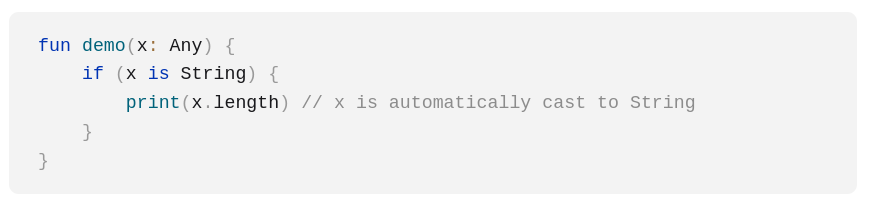
\includegraphics[width=\linewidth]{img/SmartCast.png}
    \caption{Codebeispiel zu Smart Casts\footnotemark}
\end{figure}
\footnotetext{\url{https://kotlinlang.org/docs/typecasts.html#smart-casts} letzter Zugriff: 04.01.2024}
Der Kotlin Compiler ist in der Lage den Kontext in dem der $is$ Operator auftritt zu beachten \cite{KotlinLangDoc}. Dadurch lassen sich explizite Typkonversionen und folglich potenzielle Fehler vermeiden. Dies gilt allerdings nur, wenn der Compiler ausschließen kann, dass sich die Variable $x$ nicht nach der Prüfung mit dem $is$ Operator noch ändert \cite{KotlinLangDoc}.

\subsection{Datenklassen}
Datenklassen sind eine prägnante Form von Klassen, die zum Speichern von Daten, in Form von Properties, vorgesehen sind \cite{KotlinLangDoc}. Die Abbildung 2 zeigt ein Codebeispiel zu Datenklassen. Dabei wird die Datenklasse $Person$ mit den beiden Properties $name$ und $age$ deklariert. Die Klassendeklaration in Kotlin erlaubt es den primären Konstruktor direkt im Kopf der Klasse zu deklarieren. Für Properties die im Kopf der Klasse deklariert wurden, werden implizit $get$ und $set$ Funktionen generiert \cite{KotlinLangDoc}. In diesem Fall werden die Funktionen nur für die Property $name$ generiert. Die Property $age$ wird im Rumpf der Klasse deklariert, was diese Property von der automatischen Generierung der $get$ und $set$ Funktionen ausnimmt \cite{KotlinLangDoc}.
\begin{figure}[!htb]
    \centering
    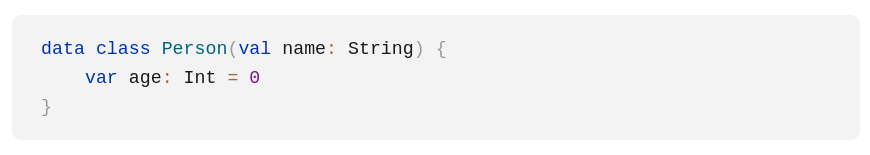
\includegraphics[width=\linewidth]{img/Dataclass.png}
    \caption{Codebeispiel zu Datenklassen\footnotemark}
\end{figure}
\footnotetext{\url{https://kotlinlang.org/docs/data-classes.html} letzter Zugriff: 04.01.2024}
\newline
Des Weiteren implementieren alle Datenklassen in Kotlin zusätzliche Funktionen, wie $equals()$, $hashCode()$, $copy()$, $componentN()$ und $toString()$. Die $equals()$ Funktion ist zum Vergleichen von Objekten. Besonders hierbei ist, dass beim Vergleichen nur die Properties beachtet werden, die auch im primären Konstruktor der Klasse aufgeführt sind \cite{KotlinLangDoc}. Mit der $copy()$ Funktion lassen sich Objekte kopieren. Zusätzlich können mit der $copy()$ Funktion, Properties der Kopie verändert werden, indem der $copy()$ Funktion Werte übergeben werden. Die Component Funktionen werden für jede Property generiert, wobei das $N$ durch eine Zahl, beginnend von 1, ersetzt wird. Die Funktionen werden nach der Reihenfolge in der die Properties deklariert wurden, nummeriert \cite{KotlinLangDoc}. Zum Beispiel würde die Property $name$ auch über die $component1()$ Funktion aufgerufen werden können. Dieses Konzept wird in Kotlin auch als Destructuring Declarations (deutsch: destrukturierende Deklarationen) bezeichnet \cite{KotlinLangDoc}.

\subsection{Destrukturierende Deklarationen}
In Kotlin bieten destrukturierende Deklarationen die Möglichkeit mehrere Variablen gleichzeitig aus einem Objekt zu deklarieren beziehungsweise zu destrukturieren. Die Reihenfolgen für die Deklaration ist abhängig von der Deklaration des primären Konstruktors \cite{KotlinLangDoc}. Die Abbildung 3 zeigt ein Codebeispiel für eine destrukturierende Deklaration. Dabei werden die Variablen $name$ und $age$ mit dem Objekt $person$ initialisiert. Das Objekt $person$ ist ein Objekt der Klasse $Person$, die in der Abbildung 2 abgebildet ist. Die Variablen werden mit den Properties von $person$ initialisert.
\begin{figure}[!htb]
    \centering
    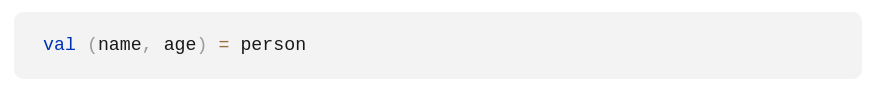
\includegraphics[width=\linewidth]{img/DestrucDecl.png}
    \caption{Codebeispiel zu destrukturierenden Deklaration\footnotemark}
\end{figure}
\newline
Ein weiteres Beispiel ist in der Abbildung 4 zu sehen. Dabei wird in der For-Schleife die destrukturierende Deklaration genutzt um durch die $key$ und $value$ Objekte einer Map zu iterieren. Diese Schreibweise vereinfacht im Allgemeinen die Iteration durch Collections.
\begin{figure}[!htb]
    \centering
    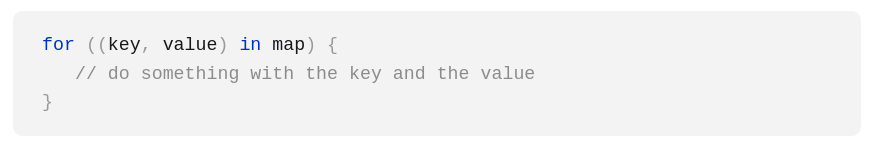
\includegraphics[width=\linewidth]{img/DestrucDecl2.png}
    \caption{Verwendung von destrukturierenden Deklarationen \footnotemark}
\end{figure}
\footnotetext{\url{https://kotlinlang.org/docs/destructuring-declarations.html} letzter Zugriff: 04.01.2024}

\subsection{Null Sicherheit}
Ein zentrales Konzept in Kotlin ist Null Sicherheit. Dabei sollen alle möglichen Ursachen für Referenzierung auf null verhindert werden \cite{KotlinLangDoc}. Kotlin bietet diesbezüglich einige Features. Wie in Kaptiel 2.1 bereits erläutert wurde, unterscheidet Kotlin zwischen nullbaren und nicht-nullbaren Typen. Das heißt unter anderem, dass der Compiler nicht kompiliert, wenn ein nicht-nullbarer Typ mit null initialisiert wird. Bei der Deklaration von Variablen können Typen explizit als nullbar deklariert werden, indem der $?$ Operator hinter der Typbezeichnung steht \cite{KotlinLangDoc}. Falls allerdings die Referenzierung auf ein Objekt eines nullbaren Typen gewünscht wird, erlaubt der Compiler dies wenn zuvor auf null, beispielsweise in einem if-Statement, geprüft wurde \cite{KotlinLangDoc}. Dies gilt nur, wenn die Variable nicht veränderbar ist \cite{KotlinLangDoc}. \newline
Eine weiteres Feature zum Unterbinden von Null Referenzierungen, sind Safe Calls (deutsch: sichere Aufrufe) \cite{KotlinLangDoc}. Dabei können beispielsweise Properties von Objekten eines nullbaren Typen versucht werden aufzurufen, ohne eine Ausnahme auszulösen. Dazu wird der $?$ Operator vor dem Punktoperator verwendet. Im Fall, dass das Objekt null ist, wird dadurch der Aufruf vorzeitig abgebrochen und zu null evaluiert. Das verhindert die Ausnahme, die anderenfalls ausgelöst werden würde. \newline
Der Elvis-Operator $?:$ wird in Kotlin auch unterstützt. Dieser lässt sich am besten als vereinfachte Schreibweise für ein if-Statement erklären. Für ein Objekt eines nullbaren Typen, prüft der Elvis Operator ob das Objekt null ist, falls das der Fall ist, soll ein alternativer Wert, der nach dem Elvis Operator steht, zurückgegeben werden. Falls das Objekt nicht null ist, wird der Wert des Objekts zurückgegeben \cite{KotlinLangDoc}. \newline
Ein weiteres Feature sind Safe Casts (deutsch: sichere Typumwandlungen) \cite{KotlinLangDoc}. Sichere Typumwandlungen sollen Ausnahmen bei der expliziten Typumwandlungen verhindern. Ein Beispiel dafür zeigt die Abbildung 5. Hierbei wird die Variable $aInt$ mit dem nullbaren Typ $Int?$ deklariert. Die Variable $aInt$ soll mit dem Wert der Variable $a$ initialisiert werden, dabei soll $a$ in den Typ $Int$ umgewandelt werden, falls $a$ nicht null ist. Im Fall, dass $a$ null ist, wird einfach null zurückgegeben \cite{KotlinLangDoc}.
\begin{figure}[!htb]
    \centering
    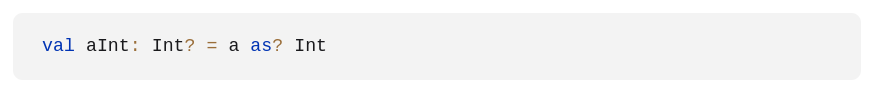
\includegraphics[width=\linewidth]{img/SafeCast.png}
    \caption{Codebeispiel zur sicheren Typumwandlung\footnotemark}
\end{figure}
\footnotetext{\url{https://kotlinlang.org/docs/null-safety.html#the-operator} letzter Zugriff: 04.01.2024}

\subsection{Higher-Order Funktionen}
Funktionen werden in Kotlin als Objekte erster Klasse behandelt \cite{KotlinLangDocHigherOrder}. Das heißt, sie lassen sich als Parameter in anderen Funktionen nutzen und können auch von einer Funktion zurückgegeben werden. Higher-Order Funktionen sind Funktionen, die andere Funktionen entweder als Parameter bekommen oder als Rückgabewert ausgeben \cite{KotlinLangDocHigherOrder}. Zum Deklarieren der Parameter und Rückgabe Funktionen, werden function types (deutsch: Funktionstypen) genutzt \cite{KotlinLangDocHigherOrder}. In Kotlin lassen sich die Funktionstypen zum Beispiel folgendermaßen ausdrücken: $(Int, String) -> Boolean$. Das Beispiel zeigt eine Funktion mit zwei Parametern, einem $Integer$ und einem $String$. Der Rückgabewert der Funktion ist ein Wert vom Typ Boolean. Häufig werden in Kotlin Higher-Order Funktionen als Extension Funktions eingebunden, um zum Beispiel bestimmte Java Bibiotheken mit hilfreichen Funktionalitäten zu erweitern (siehe Kapitel 5.4). Ein weitere Verwendung für Higher-Order Funktionen, ist das Arbeiten auf Collections\footnote{\url{https://kotlinlang.org/api/latest/jvm/stdlib/kotlin.collections/} letzter Zugriff: 06.01.2024} in Kotlin. In Kotlins Standardbibliothek werden Higher-Order Funktionen, wie $forEach()$ und $filter()$ implementiert. Mit der $forEach()$ Funktion kann über Collections iteratiert werden und dabei eine Funktion bestimmt werden, die für jede Iteration auf ein Element der Collection ausgeführt werden soll. Die $filter()$ Funktion iteriert ebenfalls über eine Collection und erhält eine Funktion die für jedes Element der Collection eine Bedingung prüft. Die Elemente der Collection, die die Bedingung erfüllen, werden von der $filter()$ als Collection zurückgegeben.
\subsection{Coroutines}
Coroutines sind ein Feature in Kotlin um effizient laufende asynchrone Programme zu schreiben. Wenn ein Thread blockiert wird, um beispielsweise auf eine Eingabe zu warten, wird der Kontext eines anderen Threads geladen, um dessen Befehle abzuarbeiten. Beim Wechseln des Kontexts entsteht immer ein erhöhter Rechenaufwand. Zudem werden für jeden Thread entsprechend Ressourcen allokiert. Somit kann sich ein häufiges Wechseln des Kontexts sich durch eine schlechtere Performance des Programms bemerkbar machen. Alternativ, können Threads auch weiter laufen ohne blockiert werden zu müssen, dies involviert Techniken der asynchronen Programmierung, wie Callbacks. Allerdings erhöht sich dadurch unweigerlich die Komplexität des Programms. Für diesen Fall gibt Coroutines. Statt einen Thread zu blockieren, sollen die Befehle eines Threads auf Coroutines verteilt werden, die unabhänig voneinander ausgeführt werden können. Coroutines können blockiert (suspendiert) werden, ohne dadurch den gesamten Thread zu blockiert. Zusätzlich sorgen Coroutines dafür, dass der Rechenaufwand durch Kontextwechsel verringert wird, ohne dabei die Lesbarkeit des Codes zu beeinträchtigen \cite{Kotlin_In-D}. \newline
Coroutines werden innerhalb eines Threads ausgeführt. Man kann sich eine Coroutine als eine Art ressourcenschonenden Thread vorstellen, der ebenfalls parallel Befehle abarbeitet, jedoch unabhängig von dem Thread in dem die Coroutine läuft. Coroutines besitzen ebenfalls wie Threads ihren eigenen Kontext, dieser ist aber in der Regel kleiner. In einem Thread können mehrere Coroutines parallel laufen. Wenn beispielsweise eine Coroutine gestoppt wird, beeinflusst dies nicht die Ausführung von anderen Coroutines in dem selben Thread. Außerdem  wird der Thread, in dem eine Coroutine gestoppt wurden, nicht gestoppt. Wird allerdings der Thread gestoppt, in dem die Coroutines existieren, werden auch die Coroutines gestoppt \cite{KotlinLangDocCoroutines}. \newline
Coroutines lassen sich in Kotlin verwenden, indem man die entsprechende Coroutines Bibliothek\footnote{\url{https://github.com/Kotlin/kotlinx.coroutines} letzter Zugriff: 05.01.2024} einbindet.  Um eine Coroutine zu starten, werden bestimmte Funktionen, wie $launch$ und $runBlocking$ (coroutine builder) verwendet. Diese müssen innerhalb eines $CoroutineScope$ aufgerufen werden. Nur auf dem $CoroutineScope$ können Coroutinen erzeugt werden. Der $CoroutineScope$ bestimmt auch die Lebensdauer der Coroutine und aller Coroutines, die innerhalb einer Coroutine erzeugt worden sind.  Das soll das Erzeugen von Coroutines strukturieren und verhindern, dass diese zu Speicherlecks führen.  Die $launch$ Funktion startet parallel eine neue Coroutine, ohne den aktuellen Thread dabei zu blockieren. Die $runBlocking$ Funktion startet eine neue Coroutine und blockiert den aktuellen Thread bis die Coroutine ausführt wurde. Außerdem erzeugt die Funktion auch einen $CoroutineScope$.
Ein wichtiges Feature sind suspending Functions (deutsch: suspendierende Funktionen). Diese erlauben es die Coroutine für eine bestimmte Zeit zu stoppen. Suspendierende Funktionen werden mit dem $suspend$ Schlüsselwort deklariert. Die Methode $delay()$ ist eine solche suspendierende Funktion. Sie kann analog zur $Thread.sleep()$ Funktion gesehen werden, allerdings nur bezogen auf das Stoppen von Coroutines. Suspendierende Funktionen lassen sich nur innerhalb einer Coroutine aufrufen. \cite{KotlinLangDocCoroutines}

\begin{figure}[!htb]
    \centering
    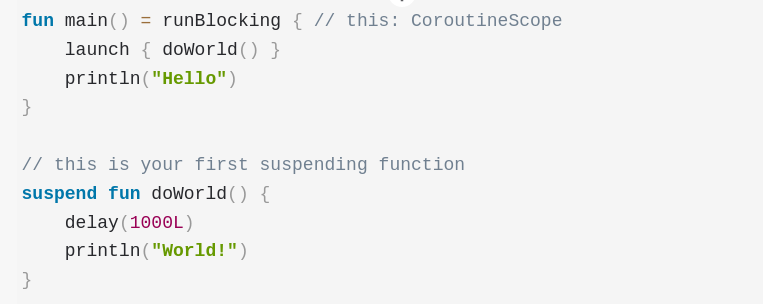
\includegraphics[width=0.9\columnwidth]{img/Coroutine.png}
    \caption{Codebeispiel zu Coroutines\footnotemark}
\end{figure}
\footnotetext{\url{https://kotlinlang.org/docs/coroutines-basics.html#scope-builder-and-concurrency} letzter Zugriff: 04.01.2024}

Die Abbildung 6 veranschaulicht wie Coroutines verwendet werden können. In dem Beispiel wird zu Beginn mit $runBlocking$ innerhalb der $main$ Funktion, der Main-Thread geblockt und eine neue Coroutine erzeugt. Innerhalb des Scopes dieser Coroutine, wird eine weitere Coroutine mit $launch$ erzeugt, die die suspendierende Funktion $doWorld()$ ausführt. Die $doWorld()$ Funktion stoppt die Coroutine für eine Sekunde und soll danach den String $"World!"$ auf die Konsole schreiben. In der Zwischenzeit wird die Coroutine in der $main()$ Funktion, weiterlaufen und den String $"Hello"$ auf die Konsole schreiben \cite{KotlinLangDocCoroutines}.
\subsection{Extensions}
In Kotlin können bestehende Klassen mithilfe von Extensions erweitert werden. Für die Erweiterung einer Klasse, muss die bestehende Klasse also nicht zwingend vererbt werden. Die Abbildung 7 zeigt ein Beispiel für die Nutzung von Extensions.  Um eine Extension Funktion zu deklarieren, wird die Funktion mit dem Bezeichner der Klasse als Prefix angegeben. In dem Beispiel wird die Klasse $MutableList$ mit der Extension Funktion $swap$ erweitert. $MutableList$ ist die Klasse zum Initialisieren von veränderbaren Listen. Die Funktion $swap$ bekommt zwei Indizes übergeben und tauscht die Position der korrespondierenden Elemente in der Liste. \newline
Extensions sind keine Erweiterung im Sinne, dass sie eine Klasse modifizieren. Extension Funktionen mit der selben Signatur wie eine bestehende Klassen-Funktion, werden beim Aufruf zugunsten der Klassen-Funktion übergangen. Extension Funktionen können aber zum Überladen von bereits existierenden Klassen-Funktionen verwendet werden. Um eine Extension außerhalb des Pakets zu nutzen, in dem die Extension deklariert wurde, muss das Paket mit der Deklaration der Extension importiert werden \cite{KotlinLangDocExtensions}.
\begin{figure}[!htb]
    \centering
    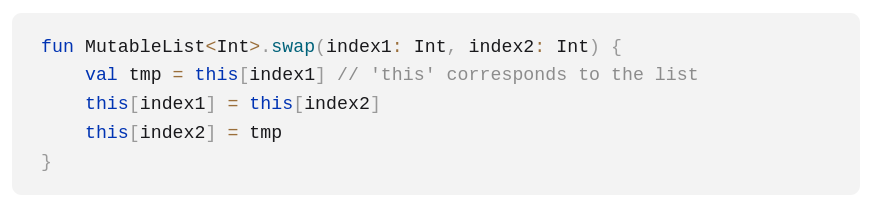
\includegraphics[width=\columnwidth]{img/Extensions.png}
    \caption{Codebeispiel zu einer Extension Funktion\footnotemark}
\end{figure}
\footnotetext{\url{https://kotlinlang.org/docs/extensions.html#extension-functions} letzter Zugriff: 04.01.2024}

\section{Verwendung von Kotlin}
Neben den bereits erwähnte Anwendungsbereichen, wie die Entwicklung für Desktop Anwendungen, bietet Kotlin auch weitere Möglichkeiten. In diesem Kapitel wird die Entwicklung von Anwendungen für Android und weitere Anwendungsbereiche vorgestellt. Zudem werden die Werkzeuge zum Erstellen von Projekte betrachtet.

\subsection{Infrastruktur}
Kotlin profitiert von den existierenden Technologien und Werkzeugen, die von JetBrains entwicklet wurden. Für das Entwickeln mit Kotlin lässt sich als Entwicklungsumgebung IntelliJ IDEA von JetBrains verwenden. Weitere Entwicklungsumgebungen wie Android Studio und Eclipse können ebenfalls verwendet werden. Ein Vorteil bei der Nutzung von IntelliJ sind die zusätzlichen Werkzeuge die mit IntelliJ gebündelt sind. Mit dem Java to Kotlin converter\footnote{\url{https://kotlinlang.org/docs/mixing-java-kotlin-intellij.html#converting-an-existing-java-file-to-kotlin-with-j2k} letzter Zugriff: 05.01.2024} (J2K) lassen sich Java Klassen direkt in Kotlin Dateien konvertieren. Ein weiteres nützliches Werkzeug, ist der IntelliJ Profiler\footnote{\url{https://www.jetbrains.com/help/idea/profiler-intro.html} letzter Zugriff: 05.01.2024}. Dieser bietet unter anderem die Möglichkeit, Projekte hinsichtlich der Speichernutzung und Laufzeit zu optimieren. Dazu bietet das Werkzeug auch die Möglichkeit zu visualisieren, wie die Speicherfreigabe durch die Garbage Collection funktioniert. \newline
Zum Builden von Projekten können Gradle oder Maven verwendet werden. Ein Vorteil bei der Nutzung von Gradle in Kotlin Projekten ist, dass Kotlin für das Schreiben der Build Skripte verwendet werden kann. Das Dokumentieren von Kotlin Code wird mit KDoc ermöglicht. KDoc funktioniert analog zur Dokumentation in Java mit Javadoc.

\subsection{Android Entwicklung}
Kotlin ist die von Google empfohlene Programmiersprache zum Entwickeln von Android Anwendungen und wird von mehr als der Hälfte aller Android Entwickler genutzt. Android bietet einige Technologien und Werkzeuge für Kotlin. Das Android GUI Framework Jetpack Compose\footnote{\url{https://developer.android.com/jetpack/compose} letzter Zugriff: 04.01.2024} kann zum Erstellen von grafischen Benutzeroberflächen genutzt werden. Das Framework selbst wurde ebenfalls in Kotlin geschrieben. Zudem bietet Android, mit AndroidKTX\footnote{\url{https://developer.android.com/kotlin/ktx} letzter Zugriff: 04.01.2024} Android-spezifische Kotlin Extensions, welche die Nutzung von Kotlin für Android mit zusätzlichen Funktionalitäten erweitert. Für die Entwicklung eignet sich Android Studio als Entwicklungsumgebung. Android Studio nutzt den Code-Editor von IntelliJ und bietet auch die Möglichkeit Java Code in Kotlin Code zu konvertieren \cite{AndroidKotlin}. \newline
Ein besonders beliebtes Feature von Kotlin für die Android Entwicklung sind Coroutines. Diese sind für die Android Entwicklung von besonderer Bedeutung, da Coroutines es vereinfachen parallelen Code auszuführen ohne den Main Thread zu blockieren. Zudem bieten Coroutines die Möglichkeit zur effizienteren Speichernutzung und führen insgesamt zu weniger Memory Leaks \cite{AndroidCoroutine}.
\subsection{Weitere Anwendungsbereiche}
Entgegen der anfänglichen Intention bei der Entwicklung von Kotlin, hat sich Kotlin über die Jahre zu einer Allzweck-Programmiersprache entwickelt. Zum Beispiel kann Kotlin auch für Data Science und Machine Learning genutzt werden. Dazu bietet Kotlin mehrere Bibiliotheken. Die DataFrame\footnote{\url{https://github.com/Kotlin/dataframe} letzter Zugriff: 05.01.2024} Bibliothek, führt passende Datenstrukturen ein, um mit dynamischen Daten arbeiten zu können. Die Bibliothek ist von der Python Bibliothek pandas\footnote{\url{https://pandas.pydata.org/} letzter Zugriff: 05.01.2024} inspiriert und die Entwicklung wird offiziell von JetBrains unterstützt. Hierfür bietet IntelliJ auch geeignete Erweiterungen. Zum Beispiel ermöglicht das Plugin Kotlin Notebook die Visualisierung von Daten in IntelliJ. Zudem lässt sich der Code auch zellenweise, ähnlich zu Juypter Notebook, ausführen \cite{KotlinLangDocData}. \newline
Des Weiteren bietet Kotlin auch die multik\footnote{\url{https://github.com/Kotlin/multik} letzter Zugriff: 05.01.2024} Bibliothek. Diese implementiert einige mathematische Funktionen und erleichtert das Arbeiten mit multidimensionalen Arrays. Somit kann die Bibliothek als Gegenstück, aber nicht in Gänze, zu Python's numpy\footnote{\url{https://numpy.org/} letzter Zugriff: 05.01.2024} gesehen werden \cite{KotlinLangDocData}. \newline
Für Deep Learning bietet Kotlin die Bibiliothek kotlindl\footnote{\url{https://github.com/Kotlin/kotlindl} letzter Zugriff: 05.01.2024}. Die Bibliothek ist von Keras\footnote{\url{https://keras.io/} letzter Zugriff: 05.01.2024} inspiriert. kotlindl ermöglicht es Deep Learning Modelle zu trainieren und enthält auch vortrainierte Modelle. Diese Bibliothek unterstützt ein begrenzte Anzahl an Deep Learning Architekturen und Schichten \cite{KotlinLangDocData}. \newline
Kotlin wird auch zum Entwickeln von serverseitigen Anwendungen verwendet. Wegen Kotlin's Java-Interoperabilität, können Technologien die auf Java basieren, einfacher in Kotlin Projekte eingebunden werden. Dazu zählt beispielsweise das Spring\footnote{\url{https://spring.io/} letzter Zugriff: 04.01.2024} Framework, welches zum Entwickeln von Web-Applikationen genutzt werden kann. JetBrains bietet auch sein eigenes Framework zum Entwickeln von Microservices und Web-Applikationen an. Dieses ist bekannt als Ktor\footnote{\url{https://github.com/ktorio/ktor} letzter Zugriff: 04.01.2024} \cite{KotlinLangDocServer}.

\subsection{Bekannte Projekte}
Eine App die Kotlin verwendet, ist Google Home\footnote{\url{https://play.google.com/store/apps/details?id=com.google.android.apps.chromecast.app&hl=de&gl=US} letzter Zugriff: 05.01.2024}. Google Home ist eine App zur Verwaltung und Steuerung von Google-Produkten und intelligenten Haushaltsgeräten. Bevor Google Kotlin zur Weiterentwicklung von Google Home eingeführt hat, wurde die App mit Java entwickelt. Ziel des Umstiegs war es, den Entwicklungsprozess produktiver zu machen. Mittlerweile ist mehr als 30\% des Google Home Codes mit Kotlin geschrieben. Aufgrund der Prägnanz von Kotlin, empfinden die Entwickler von Google Home die Entwicklung als effizienter und schneller. Der Umstieg auf Kotlin bewirkte eine deutliche Reduktion der Codezeilen. Dies wurde unter anderem durch Datenklassen und den funktionalen Features von Kotlin erzielt. Desweiteren hat Kotlins Null-Sicherheit die Anzahl an NullPointerExceptions um ungefähr 33\% verringert \cite{GoogleHome}.
\newline
Eine weitere bekannte App, die Kotlin nutzt, ist Duolingo\footnote{\url{https://play.google.com/store/apps/details?id=com.duolingo&hl=de&gl=US} letzter Zugriff: 05.01.2024}. Duolingo ist ein Lernplattform für Sprachen. Auch die Entwickler von Duolingo haben zuvor Java für ihre Android App genutzt. Der Grund für den Umstieg auf Kotlin war die wachsende Anzahl an Codezeilen, welche sich jährlich fast verdoppelt hat. Die Entwickler von Duolingo haben innerhalb von zwei Jahren ihren gesamten Java Code nach Kotlin migriert. Im Schnitt ist die Anzahl der Zeilen pro migrierte Java Klasse um 30\% gesunken. Die Migration verbesserte insgesamt die Wartbarkeit des Codes \cite{Duolingo}. \newline
Der bekannte Streaming-Dienst Netflix\footnote{\url{https://www.netflix.com/de/} letzter Zugriff: 05.01.2024} verwendet Kotlin Multiplatform für die Entwicklung einer internen Android und iOS App. Die App nennt sich Prodicle und soll den Produktionsprozess von Fernsehshows erleichtern, indem sie die Kommunikation und Zusammenarbeit der Produktionsmitarbeiter optimiert wird. Netflix hat einen großen Teil seine Anwendungslogik für beiden Plattformen entwicklet. Dies führte unweigerlich zu einem erhöhten Zeitaufwand bei Anpassungen des Codes. Der Hauptgrund weshalb Netflix sich entschieden hat Kotlin Multiplatform zu nutzen, ist um eine schneller Produktentwicklung zu ermöglichen \cite{Netflx}.

\section{Programm Implementierung}
In diesem Kapitel werden der Aufbau des Projekts und die Besonderheiten bei der Implementierung dargelegt.
\subsection{Projektaufbau}
Als Build System wurde Gradle verwendet. Das Projekt ist in drei Dateien unterteilt. Die $App.kt$ Datei beinhaltet die Implementierung des Command Line Interfaces. Die $Searcher.kt$ Datei beinhaltet die wesentliche Logik des Programms. Gemeint ist damit die rekursive Dateisuche, die Suche nach regulären Ausdrücken, die kontextbasierte Suche, sowie ein paar Hilfsfunktionen. Die $PrintHelper.kt$ Datei wird für das Formatieren und Ausgeben der Suchergebnisse genutzt.
\subsection{Command Line Interface}
Für die Umsetzung des Command Line Interfaces, wurde die Bibliothek clikt\footnote{\url{https://ajalt.github.io/clikt/} letzter Zugriff: 05.01.2024} verwendet. Zwar bietet JetBrains seine eigene Bibliothek\footnote{\url{https://github.com/Kotlin/kotlinx-cli} letzter Zugriff: 05.01.2024} an, diese wird allerdings nicht mehr aktiv weiterentwickelt. Um das Command Line Interface nutzen zu können, muss man eine Klasse erstellen, die von der abstrakten Klasse $CliktCommand$ erbt. Innerhalb der Klasse lassen sich die Optionen und Argumente definieren. Diese werden mittels Property delegates umgesetzt \cite{clikt}. Die Abbildung 8 veranschaulicht den Aufbau einer $CliktCommand$ Klasse. Das Schlüsselwort $by$ gibt an, dass die Funktion rechts daneben die Initialisierung der Property übernimmt \cite{KotlinLangDoc}. Solche Funktionen werden auch als $delgate$ (deutsch: Delegat) bezeichnet \cite{KotlinLangDoc}.
\newline In Hinblick auf das Beispiel in der Abbildung 8, ist die Funktion $option()$ und $argument()$ jeweils ein Delegat. Beide übernehmen die Zuweisung der geparsten Command Line Argumente.
\begin{figure}[!htb]
    \centering
    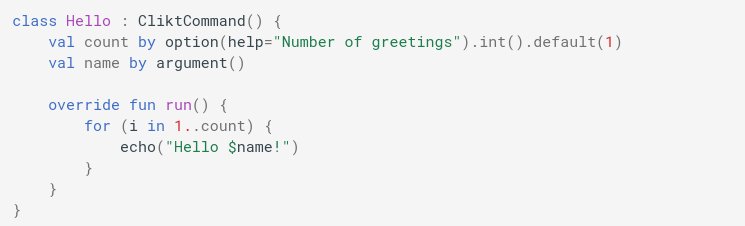
\includegraphics[width=\linewidth]{img/CliktCommand.png}
    \caption{Codebeispiel zu einem CliktCommand\footnotemark}
\end{figure}
\footnotetext{\url{https://ajalt.github.io/clikt/quickstart/} letzter Zugriff: 04.01.2024}
Klassen die von $CliktCommand$ erben, parsen die Command Line Argumente durch das Aufrufen der $main()$ Funktion. Wenn das Parsen erfolgreich war, wird die $run()$ Funktion der Klasse aufgerufen. In der $run()$ Funktion lassen sich die vorgesehene Funktionalität des Commands einbinden.
\subsection{Rekursive Dateisuche}
Für die Implementierung der rekursiven Dateisuche, wurde das Paket $kotlin.io.path$ eingebunden. Dieses unterstützt mehrere hilfreiche Funktionen zum Prüfen von Dateien im Dateisystem. Diese sind genauer gesagt Extensions der $Path$ Klasse des $java.nio.file$ Paketes. Die Extension Funktionen lassen sich auf einem $Path$ Objekt aufrufen. Das Kotlin Paket bietet Extension Funktionen zum Prüfen auf reguläre und versteckte Dateien, sowie auch eine Funktion zum Prüfen auf Verzeichnisse. Zudem enthält das Paket auch eine Funktion, die alle Einträge in einem Verzeichnis als Liste von $Path$ Objekten zurückgibt. \newline
Die Funktion zum Erkennen von Binärdateien basierend auf einem Algorithmus\footnote{\url{https://stackoverflow.com/questions/620993/determining-binary-text-file-type-in-java} letzter Zugriff: 06.01.2024}, der die ASCII Zeichen einer Datei untersucht. Der Algorithmus beruht auf der Annahme dass, Binärdateien typischerweise vermehrt Steuerzeichen und ASCII Zeichen aus dem Erweiterten ASCII Zeichen Satz\footnote{\url{https://theasciicode.com.ar/} letzter Zugriff: 05.01.2024} beinhalten. Der Algorithmus nimmt sich hierfür 1024 Bytes einer Datei und zählt die typischen und untypische ASCII Zeichen. Falls der prozentuale Anteil der typischen ASCII Zeichen über 50\% beträgt, wird die Datei als Binärdatei betrachtet.
\subsection{Suchen von regulären Ausdrücken}
Für die Iteration durch die Textzeilen einer Datei wurden die Klassen $InputStream$ und $File$\footnote{\url{https://kotlinlang.org/api/latest/jvm/stdlib/kotlin.io/java.io.-file/} letzter Zugriff: 05.01.2024} aus dem Java Paket $java.io$ eingebunden. Beide Klassen werden in Kotlin durch Extension Funktionen erweitert. Mit der Extension Funktion $bufferedReader()$ auf einem $InputStream$ Objekt, welches eine Textdatei repräsentiert, lässt sich ein Objekt der Klasse $BufferedReader$ erzeugt. Dieses ist notwendig, um durch den Inhalt der Datei zu iterieren. Auf dem $BufferedReader$ Objekt, lässt sich dann die Extension Funktion $forEachLine()$ aufrufen. Diese Funktion ist eine Higher-Order Funktion und iteriert durch jede Zeile der Textdatei. Als Parameter erhält $forEachLine()$ unter anderem eine Funktion mit der aktuellen Textzeile als Parameter und dem Rückgabewert $Unit$ (in Java $void$). Diese Funktion erlaubt es die Textzeile zu verarbeiten. \newline
Für die Umsetzung der Suche von reguläre Ausdrücken, wurde das Paket $java.util.regex$ verwendet. Das Paket enthält eine Klasse $Pattern$, die einen String in einen reguläre Ausdruck kompilieren kann. Ein Objekt der Klasse $Pattern$ wurde genutzt, um das eingegebene Suchmuster zu einem regulären Ausdruck zu kompilieren. Mit dem $Pattern$ Objekt und einer $CharSequence$ lässt sich ein $Matcher$ Objekt erzeugen. Die $CharSequence$ ist in diesem Fall eine einzelne Textzeilen aus einer Datei. Mit der $find()$ Funktion auf dem $Matcher$ Objekt, lassen sich alle Übereinstimmungen zwischen der Textzeile und dem regulären Ausdruck finden. Zusätzlich speichert das $Matcher$ Objekt die Indizes der übereinstimmenden Stellen. Dies wurde benötigt, um die Färbung der Ausgabe zu realisieren.
\subsection{Hilfreiche Konzepte und Erkenntnisse}
Während der Implementierung des Programms, haben sich ein paar Konzepte von Kotlin als besonders hilfreich erwiesen. Zum einen wurde die Eingabe des Nutzers mithilfe von Kotlins Datenklassen modelliert. Dadurch konnte der insgesamt benötigte Code deutlich reduziert werden, da $get$ und $set$ Funktionen nicht separat deklariert werden mussten. Des Weiteren hat sich die Java Interoperabilität bei der Entwicklung bemerkbar gemacht. Alle Java Bibliotheken, können auf Wunsch im Kotlin Projekt genutzt werden. Die für die rekursive Dateisuche genutzte $Path$ Klasse aus einem Java Paket, besitzt Extension Funktionen die durch ein Kotlin Paket verfügbar sind. Diese wurden für das Prüfen von Dateien im Dateisystem genutzt. Dadurch wurde Implementierung der rekursive Suche deutlich vereinfacht. Weitere Features die verwendet worden sind, sind die Features zur Null-Sicherheit. Darunter wurde der Elvis Operator zum Initialisieren von Variablen genutzt. Hinsichtlich der Ausgabe der Suchergebnisse, bietet Kotlin auch eine sehr prägnante String Formatierung an. \newline
Der integrierte Code Analyse Assistent von IntelliJ vereinfachte, das Einhalten von Kotlin spezifische Konventionen. Zudem bietet der Assistent auch an, bestimmte Ausdrücke kürzer zu fassen. So wurden zum Beispiel when-Statements, Kotlins Äquivalent eines switch Statements, auf Hinweis des Assistenten in eine zuweisende Anweisungen umgeschrieben. Dadurch ließ sich wiederholender Code reduzieren. Außerdem bietet der Code Analyse Assistent, auch die Möglichkeit, geschriebenen Java Code innerhalb einer Kotlin Datei in Kotlin Code zu konvertieren. Dies wurde bei der Einbindung des Algorithmus zum Prüfung von Binärdateien angewendet. Der Assistent konvertiert den Java Code auf Wunsch vollständig automatisch.\newline
Insgesamt, hat die Entwicklung des Projekts mit Kotlin, die allgemeinen Stärken der Programmiersprache verdeutlicht. Kotlin benötigt durch Konzepte wie Datenklassen, merkbar weniger Codezeilen. Die Interoperabilität mit Java erleichterte die Implementierung, da Java Bibliotheken einfach eingebunden werden konnten. Besonders hilfreich waren die von Kotlin implementierten Extension Funktionen für bestehende Java Pakete. Durch Higher-Order Funktionen wurde das Iterieren durch die Dateien auch vereinfacht.
\section{Fazit}
Kotlin ist eine von JetBrains entwicklete Programmiersprache, die statisch typisiert ist und moderne Programmierparadigmen zusammen mit bekannte Programmierkonzepten aus Java vereint. Kotlin läuft auf der JVM und anderen Plattformen. Die ursprüngliche Intention hinter der Entwicklung war es, eine Alternative zu Java zu schaffen. Die wesentlichen Schwächen von Java, aus Sicht von JetBrains, sind die mangelnde Null- und Typ-Sicherheit und die mangelnde Prägnanz. Kotlin bietet diesbezüglich zahlreiche Features wie Higher-Order Funktionen, Safe Calls, Datenklassen und Extensions, um diese Schwächen zu beseitigen. Mit Extensions werden in Kotlin unter anderem die Funktionalitäten von existierenden Java Bibliotheken erweitert. Des Weiteren sorgt die Typinferenz in Kotlin für eine kürzere und leicht verständliche Syntax. Kotlin wird hauptsächlich für die Android Entwicklung genutzt. Es lässt sich auch für andere Anwendungsbereiche einsetzen, wie zum Beispiel für Desktop- oder serverbasierte Anwendungen. Ein wesentliches Feature ist, dass Kotlin vollständig mit Java interoperieren kann. Sämtliche Java Bibliotheken, lassen sich somit uneingeschränkt in Kotlin Projekten verwenden. Bekannte Unternehmen, wie Google und Netflix, haben aus diesem Grund Kotlin in ihre Projekte integriert. Ein weiteres besonderes Konzept von Kotlin sind Coroutines, welche die Implementierung von performanten asynchronen Applikationen ermöglichen. Kotlin profitiert außerdem vom JetBrains Ökosystem, indem es Werkzeuge wie IntelliJ IDEA für die Entwicklung nutzen kann.

\bibliographystyle{unsrt}
\bibliography{references}

\end{document}
